\documentclass[journal]{IEEEtran}
\usepackage{cite}
\usepackage{amsmath,amssymb}
\usepackage{graphicx}
\usepackage{booktabs}
\usepackage{textcomp}
\usepackage{url}
\def\UrlFont{\footnotesize\ttfamily}

\begin{document}

\title{Federated Intrusion Detection Under\\ Label-Flipping Poisoning on CICIoT2023}

\author{Salvador~Leon~Lopez, Elena~Victoria~Sanchez, Joe~Reyna, and~April~Flores%
\thanks{The authors are Group 8 in CSCI 6330: Foundations of Intelligent Security Systems, Department of Computer Science, The University of Texas Rio Grande Valley.}%
\thanks{Milestone 2 progress report, November 2026. Code: github.com/Jreyna4/CSCI-6330-Foundation-Security-Systems-Course-Project.}}

\markboth{CSCI 6330 Course Project, Milestone 2, Fall 2026}%
{Leon Lopez \MakeLowercase{\textit{et al.}}: Federated Intrusion Detection Under Label-Flipping Poisoning}

\maketitle

\begin{abstract}
We simulate a ten-client federated intrusion detector on CICIoT2023 (all 63 files, 306,124 flows) and measure what label-flipping clients cost and whether robust aggregation recovers it, with five paired seeds, six aggregation rules and ten robustness checks. One attacker relabeling half of its attack rows as benign lowers FedAvg's macro F1 by only $1.1\pm0.4$ points, so H1 (3 points) is not supported, and trimmed mean does not recover it (H2 not supported). Macro F1 hides the damage: missed attacks rise from 7.1\% to 10.5\%, almost all in four families that resemble benign traffic, and a Recon-only attack leaves macro F1 unchanged while doubling missed Recon. Damage follows the number of poisoned rows, not attacker size. The defenses detect the attacker but help clearly only against strong attacks.
\end{abstract}

\begin{IEEEkeywords}
Federated learning, intrusion detection, data poisoning, label flipping, robust aggregation, CICIoT2023.
\end{IEEEkeywords}

\begin{table*}[t]
\caption{Grouped split (whole files) and per-family supports}
\label{tab:split}
\centering\footnotesize
\setlength{\tabcolsep}{6pt}
\begin{tabular}{@{}lrrrrrrrrrrr@{}}
\toprule
Split & Files & Rows & Share & Benign & DDoS & DoS & Recon & Web & BruteForce & Spoofing & Mirai \\
\midrule
Train & 44 & 214,725 & 70.1\% & 31,434 & 31,443 & 31,335 & 31,648 & 16,791 & 8,941 & 31,730 & 31,403 \\
Val & 6 & 30,045 & 9.8\% & 4,375 & 4,505 & 4,525 & 4,253 & 2,468 & 1,301 & 4,312 & 4,306 \\
Test & 13 & 61,354 & 20.0\% & 9,191 & 9,052 & 9,140 & 9,099 & 4,356 & 2,267 & 8,958 & 9,291 \\
\bottomrule
\end{tabular}
\end{table*}

\section{Research Question and Changes}
\IEEEPARstart{O}{rganizations} that see different attack traffic could train a shared intrusion detector with federated learning (FL) \cite{mcmahan2017} without pooling raw captures, but the server cannot inspect client data, so a compromised client can poison the model \cite{tolpegin2020}.
\emph{RQ:} in a ten-client federated IDS on non-IID partitions of CICIoT2023 \cite{neto2023}, how much detection performance is lost when one client flips labels, and does coordinate-wise trimmed mean \cite{yin2018} recover it?
\emph{Hypotheses:} (H1) FedAvg macro F1 falls by more than 3 points versus the paired clean run; (H2) trimmed mean recovers at least half of that loss.

\emph{Changes after Milestone 1 feedback:} a documented grouped split with per-family supports (Sec.~\ref{sec:split}); the 46$\rightarrow$39 feature mapping (Table~\ref{tab:features}); an \emph{unweighted-mean} control; definitions of label-informed held-out assignment and PR-AUC (Sec.~\ref{sec:metrics}); and the paired comparison and per-family/per-client error analysis first, as requested. We also added three defenses, attackers of different sizes, attack strength, a targeted attack and update diagnostics (Sec.~\ref{sec:checks}).

\section{Data and Experimental Design}

\subsection{Subset}
We read all 63 MERGED\_CSV files (45,019,234 rows; 9 rows with an empty label dropped). From each file we sample at most 1,429 rows per family (575,321 rows), then remove 19 inf/NaN rows, 27,282 exact (feature+label) duplicates and 14,033 rows whose features occur with conflicting labels, \emph{before} splitting. Each family is capped at 45,000 rows; Web (23,615) and BruteForce (12,509) are kept whole. The subset has 306,124 rows; its family prevalence is a design choice (raw DDoS is 72.3\%, subset 14.7\%).

\subsection{Grouped split}\label{sec:split}
Each source file goes entirely into one split, so fractions move in steps of about $1/63 \approx 1.6\%$ of the rows (the Milestone~1 pilot's 12 files gave 8.3\% steps, hence 74.4/8.5/17.0\%). Of 2,000 seeded file assignments we keep the one closest to 70/10/20 and to the overall family mix (Table~\ref{tab:split}); the file list and per-file counts are in \texttt{split\_files.csv}.

\emph{Limitation.} Every file contains all eight families, so one capture can span several files, and the release has no capture id, IP or timestamp to group on. A nearest-neighbour check confirms this: test rows are as close to their nearest training row (median 0.120, standardized features) as training rows are to each other (0.131). Results measure generalization within one testbed, not to unseen captures.



\subsection{Features}
The documentation lists 46 flow features; our release has 39 (Table~\ref{tab:features}), checked on every run (\texttt{feature\_schema.csv}). We do no feature selection: none of the 39 is an identifier (no IPs, ports, MACs or timestamps), the 8 missing ones are not in the files, and selecting on our own data would add a leakage-prone tuning step. Each feature gets $\mathrm{sign}(x)\log(1+|x|)$ (heavy-tailed counts and rates), then standardization fit on the training pool. Removing IAT, a possible timing shortcut, at model input (same rows and clients) leaves centralized macro F1 unchanged (.742 both ways).

\begin{table}[t]
\caption{Official 46 features $\rightarrow$ 39 model inputs}
\label{tab:features}
\centering\footnotesize
\begin{tabular}{@{}p{0.26\columnwidth}p{0.66\columnwidth}@{}}
\toprule
Status & Features \\
\midrule
Kept (37) & Header\_Length, Protocol Type, Rate, 7 flag numbers, ack/syn/fin/rst counts, HTTP, HTTPS, DNS, Telnet, SMTP, SSH, IRC, TCP, UDP, DHCP, ARP, ICMP, IPv, LLC, Tot sum, Min, Max, AVG, Std, Tot size, IAT, Number, Variance \\
Renamed (1) & Duration (TTL) $\rightarrow$ Time\_To\_Live \\
Added (1) & IGMP \\
Not in release (8) & flow\_duration, Srate, Drate, urg\_count, Magnitue, Radius, Covariance, Weight \\
\bottomrule
\end{tabular}
\end{table}

\subsection{Clients and attacker}
Ten clients are formed by Dirichlet label skew ($\alpha=0.5$) \cite{hsu2019}. Automatic checks (share $\geq$2\%, size ratio $\leq$20, purity $\leq$95\%, $\geq$2 families with $\geq$50 rows) pass for Dirichlet (11,262--31,560 rows; max purity 0.83) and IID, and fail for k-means again (175--49,318 rows; one client 99.9\% one family), so Dirichlet stays primary, as in Milestone~1. The attacker is fixed: the client with the most attack rows, here client~5 (31,560 rows, 14.7\% of the pool, mostly Spoofing and DDoS). Per seed it relabels a fixed 50\% of each of its attack families as Benign (about 15,460 rows, 7.2\% of the pool) and otherwise trains honestly.

Held-out rows are assigned to clients with the frozen per-family Dirichlet proportions, i.e.\ using their \emph{labels}: label-informed benchmark construction, not a client-identification rule, acceptable because labels are never model inputs and the test set is never used for tuning.



\begin{figure*}[t]
\centering
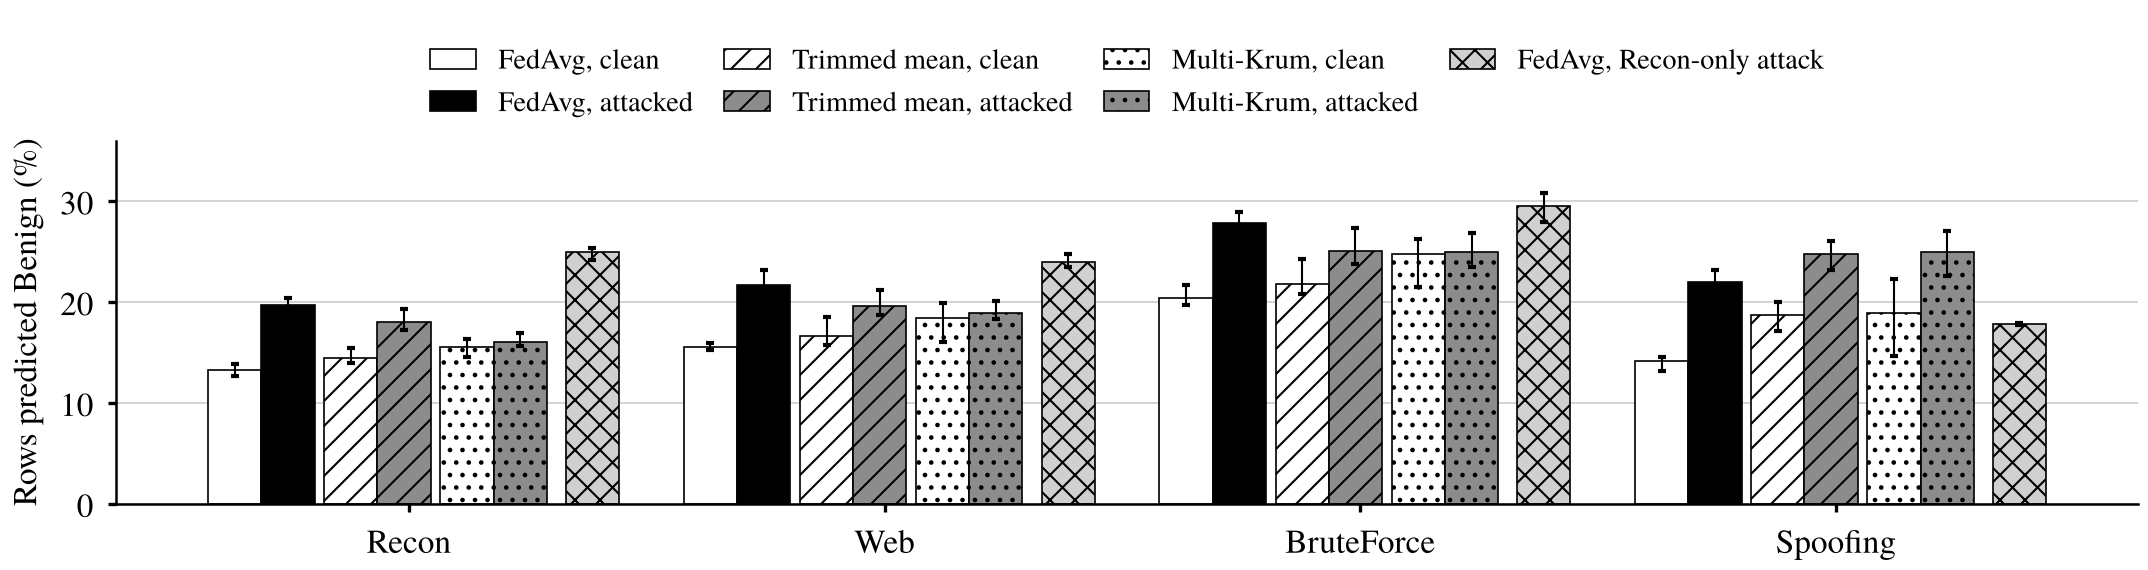
\includegraphics[width=\textwidth]{families_benign.png}
\caption{Share of each family's validation rows predicted Benign (mean over 5 seeds, 3 for the Recon-only attack; bars show the range). DDoS, DoS and Mirai are essentially never predicted Benign ($\leq$0.02\%) and are omitted.}
\label{fig:families}
\end{figure*}

\section{Methodology}
\emph{Model and training} (unchanged, identical in every condition): MLP 39--128--64--8 (ReLU, dropout 0.1; 13,896 parameters), Adam (lr $10^{-3}$), batch 256, cross-entropy; 30 FL rounds of one local epoch with all ten clients in our own simulation loop (Flower \cite{beutel2020} deprecated its simulation API). Each round moves 1.11\,MB (33.4\,MB per run); a run takes about 33\,s on a MacBook Pro CPU (Python 3.14, PyTorch 2.14).

\emph{Aggregation.} FedAvg weights client models by size; the \emph{unweighted mean} does not, so FedAvg$\rightarrow$mean isolates weighting. Two per-coordinate rules: trimmed mean ($\beta=0.2$: drop the 2 highest and 2 lowest of 10 values, average 6) and the coordinate-wise median. Two whole-update rules \cite{blanchard2017}: Krum keeps the one client whose update is closest to its neighbours, and multi-Krum averages the 8 most typical ($f=2$). With 3 attackers, attacker values can survive per-coordinate trimming, so that case is a stress test.

\emph{Design and pairing.} Centralized, FedAvg on IID clients, and the six rules on Dirichlet clients, clean and attacked (Table~\ref{tab:results}), each with five run seeds (42--46); robustness checks use seeds 42--44. The data seed fixes subset, split and partition; run seeds change initialization, batch order and poisoned rows, and same-seed runs start from identical weights, so effects are paired differences (mean $\pm$ std). Each round we also log, per client, the share of its parameters that fall in the trimmed tails, its distance to the median update and its Krum rank. All results are on validation data; the test set is used once, at the end.

\subsection{Metrics}\label{sec:metrics}
\emph{Macro F1} averages per-family F1 over families with at least one true row. \emph{Per-family PR-AUC} is one-vs-rest average precision with that family's softmax probability as the score; \emph{macro PR-AUC} averages it over families with at least one positive and one negative row. Families with no support are excluded and listed, never scored 0 or 1, which matters for small per-client held-out sets. We also report the binary miss rate (FNR) and false-alarm rate (FPR), per-family share of rows predicted Benign (the attacker's target), and per-client metrics on each client's held-out rows.

\section{Preliminary Results}

\begin{table}[t]
\caption{Validation results, mean over 5 seeds; $\Delta$ = paired change under attack (points, mean $\pm$ std)}
\label{tab:results}
\centering\footnotesize
\setlength{\tabcolsep}{2.6pt}
\begin{tabular}{@{}lccccc@{}}
\toprule
& \multicolumn{3}{c}{Macro F1} & \multicolumn{2}{c}{Missed attacks (\%)} \\
\cmidrule(lr){2-4}\cmidrule(l){5-6}
Rule & Clean & Attacked & $\Delta$ & Clean & $\Delta$ \\
\midrule
Centralized & .742 & -- & -- & 6.9 & -- \\
FedAvg, IID & .710 & -- & -- & 7.5 & -- \\
\midrule
FedAvg & .693 & .682 & $-1.1\pm0.4$ & 7.1 & $+3.4\pm0.2$ \\
Unweighted mean & .691 & .683 & $-0.8\pm0.2$ & 8.1 & $+2.3\pm0.3$ \\
Trimmed mean & .689 & .678 & $-1.1\pm0.3$ & 8.2 & $+2.1\pm0.1$ \\
Median & .688 & .676 & $-1.2\pm0.4$ & 8.4 & $+2.1\pm0.4$ \\
Krum & .629 & .612 & $-1.7\pm1.3$ & 11.5 & $+1.9\pm3.6$ \\
Multi-Krum & .666 & .680 & $+1.4\pm2.0$ & 8.8 & $+1.2\pm1.2$ \\
\bottomrule
\end{tabular}
\end{table}

\emph{Global effect.} Federated training costs 3.2 macro-F1 points against centralized training (IID) and label skew another 1.7 (Table~\ref{tab:results}). The attacker lowers FedAvg's macro F1 by $1.09\pm0.37$ points (0.72--1.62 over five seeds), so \textbf{H1 is not supported}. Trimmed mean ends $0.43\pm0.21$ points \emph{below} FedAvg under attack, so \textbf{H2 is not supported} either. Macro F1 understates the attack: missed attacks rise from 7.1\% to 10.5\% (+48\% relative) while false alarms fall from 25.4\% to 17.6\%; the attack moves the boundary toward Benign, and the two errors partly cancel in F1.

\emph{Defenses.} Under attack, dropping size weighting changes macro F1 by $+0.14\pm0.31$ points and trimming on top by $-0.57\pm0.20$. Every robust rule raises missed attacks less than FedAvg, but mainly because its clean miss rate is already higher (8.1--8.8\% vs.\ 7.1\%): under attack FedAvg, the unweighted mean, trimmed mean and median all end at 10.3--10.5\%. Krum, which keeps a single client, is poor even clean (.629). Multi-Krum has the smallest increase but its clean runs vary by $\pm$2 F1 points across seeds, so its apparent F1 \emph{gain} under attack is not reliable.

\emph{Per family and client.} The attack hits exactly the families that resemble benign traffic (Fig.~\ref{fig:families}): under FedAvg, rows predicted Benign rise from 13.2 to 19.8\% (Recon), 15.5 to 21.7\% (Web), 20.4 to 27.8\% (BruteForce) and 14.2 to 22.0\% (Spoofing). BruteForce, of which the attacker holds only 154 rows, rises almost as much as Spoofing, its largest family: the shared benign boundary shifts. Unweighted mean, trimmed mean and multi-Krum all leave Spoofing \emph{worse} than FedAvg (24.7--25.0\%). Every client's held-out miss rate rises (by 0.7--6.5 points, mean 3.6); the largest increases are at clients 1, 4 and 8, whose traffic is mostly Recon, Web and BruteForce, not at the attacker.

\emph{Why the defenses do not help.} The attacker \emph{is} detected: it ranks as the least typical client in Krum almost every round (mean rank 8.9 of 9), and 68\% of its parameters fall in the trimmed tails (37\% for honest clients). But trimming still passes about a third of them, and it also trims honest but unusual clients: client~0 has 61\% of its parameters in the tails with no attack. Removing the attacker entirely (multi-Krum) also removes the half of all Spoofing training data it holds, so Spoofing gets worse.

\subsection{Robustness checks}\label{sec:checks}
\begin{table}[t]
\caption{Robustness checks: paired change under attack, macro F1 / missed attacks (points; 3 seeds; main and no-IAT rows: 5 seeds)}
\label{tab:checks}
\centering\scriptsize
\setlength{\tabcolsep}{2.2pt}
\begin{tabular}{@{}lcccc@{}}
\toprule
Setting & FedAvg & Unw.\ mean & Trimmed & Multi-Krum \\
\midrule
Main: client 5, 50\% & $-1.1$/$+3.4$ & $-0.8$/$+2.3$ & $-1.1$/$+2.1$ & $+1.4$/$+1.2$ \\
Typical-size attacker (0) & $-1.4$/$+2.9$ & $-1.0$/$+3.2$ & $-0.6$/$+2.0$ & $-2.6$/$+1.2$ \\
Random attackers (6, 2, 3)$^a$ & $-0.5$/$+1.0$ & $-0.7$/$+1.8$ & $-0.5$/$+1.3$ & $-0.5$/$+0.4$ \\
25\% of rows flipped & $-0.6$/$+1.6$ & -- & $-0.8$/$+1.2$ & $+0.5$/$+1.8$ \\
100\% of rows flipped & $\mathbf{-4.7}$/$\mathbf{+11.2}$ & -- & $-2.1$/$+4.0$ & $+0.5$/$+1.9$ \\
Recon$\rightarrow$Benign only (1) & $+0.0$/$+3.8$ & $-0.6$/$+3.6$ & $-0.4$/$+3.3$ & $-0.8$/$+1.1$ \\
2 attackers (5, 9) & $-2.5$/$+7.4$ & $-1.8$/$+5.0$ & $-2.0$/$+4.2$ & -- \\
3 attackers (5, 7, 9)$^b$ & $-4.1$/$+11.5$ & $-2.8$/$+7.4$ & $-3.4$/$+7.3$ & -- \\
20 clients, 2 attackers & $-1.2$/$+2.8$ & $-0.6$/$+1.3$ & $-1.0$/$+1.0$ & $+0.4$/$+1.6$ \\
60 rounds & $-1.0$/$+2.8$ & -- & $-1.2$/$+1.8$ & -- \\
Class-balanced loss & $-0.3$/$+3.3$ & -- & $-1.0$/$+1.8$ & $-2.5$/$-1.5$ \\
No IAT feature & $-1.1$/$+4.1$ & -- & -- & -- \\
\bottomrule
\multicolumn{5}{@{}p{0.98\columnwidth}@{}}{$^a$Mean of three seeded draws. $^b$Stress test: more attackers than values trimmed per side. Numbers in parentheses: attacking clients.}
\end{tabular}
\end{table}
\emph{Attacker size vs.\ poisoning.} Our main attacker is also the largest client. A typical-sized attacker (client~0, 22,711 rows) does almost the same damage ($+2.9$ points missed), while randomly drawn clients do much less ($+0.7$ to $+1.3$). Client~3 is larger than client~0 but holds 22\% fewer attack rows and does a third of the damage: \emph{damage follows the number of poisoned rows, not client size} (Table~\ref{tab:checks}).

\emph{Attack strength and targeting.} Flipping 25, 50 and 100\% of the attacker's attack rows costs FedAvg 0.6, 1.1 and 4.7 points, so H1's threshold is crossed only by the strongest attack. There the defenses do help: trimmed mean cuts the increase in missed attacks from $+11.2$ to $+4.0$ points and multi-Krum to $+1.9$. A Recon-only attack (client~1, all its Recon rows) leaves macro F1 unchanged ($+0.01$) while Recon rows predicted Benign rise from 13\% to 25\% (Fig.~\ref{fig:families}); multi-Krum holds Recon at 16\%, trimmed mean at 23\%.

\emph{Other checks.} More attackers raise the damage steadily (stress test at 3). Twenty clients, 60 rounds, removing IAT and a class-balanced loss (which raises BruteForce recall from 43\% to 63\%) all leave the attack's effect on FedAvg at $+2.8$ to $+4.1$ points of missed attacks.

\section{Discussion and Next Steps}
With nine honest clients holding 85\% of the data, a mild label flip shifts the benign boundary rather than breaking the model, and macro F1 barely registers it; a targeted flip is invisible to it. Robust rules detect the attacker but only help clearly when the attack is strong, because per-coordinate trimming lets part of the attacker through and removes honest outliers, while removing whole clients also removes their honest data. The pilot's 12-point loss reflected its small subset and 5 rounds.

\emph{Next (final report):} more seeds for multi-Krum, defenses that down-weight rather than drop suspicious clients, and one final test-set evaluation. \emph{Limitations:} one testbed with simulated clients; files are not independent captures; capped prevalence; label flipping only.

\begin{thebibliography}{00}
\itemsep 0pt
\bibitem{mcmahan2017} B. McMahan \emph{et al.}, ``Communication-efficient learning of deep networks from decentralized data,'' \emph{Proc. AISTATS}, 2017.
\bibitem{tolpegin2020} V. Tolpegin, S. Truex, M. E. Gursoy, and L. Liu, ``Data poisoning attacks against federated learning systems,'' \emph{Proc. ESORICS}, 2020.
\bibitem{neto2023} E. C. P. Neto \emph{et al.}, ``CICIoT2023: A real-time dataset and benchmark for large-scale attacks in IoT environment,'' \emph{Sensors}, vol.~23, no.~13, 2023.
\bibitem{yin2018} D. Yin, Y. Chen, K. Ramchandran, and P. Bartlett, ``Byzantine-robust distributed learning,'' \emph{Proc. ICML}, 2018.
\bibitem{hsu2019} T.-M. H. Hsu, H. Qi, and M. Brown, ``Measuring the effects of non-identical data distribution for federated visual classification,'' arXiv:1909.06335, 2019.
\bibitem{blanchard2017} P. Blanchard, E. M. El Mhamdi, R. Guerraoui, and J. Stainer, ``Machine learning with adversaries: Byzantine tolerant gradient descent,'' \emph{Proc. NeurIPS}, 2017.
\bibitem{beutel2020} D. J. Beutel \emph{et al.}, ``Flower: A friendly federated learning framework,'' arXiv:2007.14390, 2020.
\end{thebibliography}

\end{document}
